\externaldocument{text-02-teoreticka}

\subsection{Klasifikace objektů pomocí strojového učení}\label{subsec:klasifikace-objektu-pomoci-strojoveho-uceni}

\subsubsection{Úvod do problematiky}
V posledních letech došlo k významnému pokroku v oblasti strojového vidění, což umožňuje efektivní a přesné rozpoznávání objektů v různých prostředích.
Jednou z nejmodernějších knihoven, která si získala širokou popularitu, je YOLOv8 (You Only Look Once version 8).
Tato knihovna přináší rychlé a přesné metody detekce objektů a je ideální pro implementaci v reálném čase.
V této sekci se zaměříme na to, jak využít YOLOv8 ke specifickému úkolu: rozpoznávání slepic v kurníku.
Automatizované rozpoznávání umožňuje sledování počtu slepic.
Použití YOLOv8 přináší následující výhody:

\begin{enumerate}
    \item Rychlost a Přesnost: YOLOv8 je navrženo pro rychlou detekci objektů s vysokou mírou přesnosti, což je ideální pro aplikování v reálném čase na farmách.
    \item Jednoduchost Implementace: Díky snadnému rozhraní a rozsáhlé dokumentaci je integrace YOLOv8 do existujících systémů velmi přímočará.
    \item Flexibilita: Můžete trénovat model na vlastním datasetu slepic, což zajistí optimální rozpoznávání i v specifických podmínkách vašeho kurníku.
\end{enumerate}
V následujících sekcích si podrobně projdeme kroky, jak připravit dataset, trénovat vlastní model se zaměřením na rozpoznávání slepic a jak jej implementovat do našeho systému monitorování.

\subsubsection{Obrázkový dataset}

Obrázkový dataset je strukturovaná kolekce obrazových dat, která se používána pro potřeby strojového učení a počítačového vidění.
Tyto datasety obsahují jednotlivé obrázky, které jsou často spojeny s dodatečnými informacemi nebo anotacemi, jež jsou potřebné pro trénink modelů.
Níže jsou uvedeny hlavní aspekty, které charakterizují obrázkové datasety:

\begin{enumerate}
    \item Obrázky: Základní komponentou datasetu jsou samotné snímky, které mohou být v různých formátech (např. JPEG, PNG). Rozlišení a počet barev se může lišit v závislosti na účelu datasetu.
    \item Anotace: Kromě samotných obrázků obsahují datasety take anotace. Tyto anotace zahrnují následující informace
    \begin{itemize}
        \item Klasifikační štítky: Které identifikují, co se na obrázku nachází (např. „kočka“, „pes“, „slepice“).
        \item Ohraničující boxy: Které označují polohu specifických objektů na obrázku.
    \end{itemize}
\end{enumerate}

Datasety jsou klíčové pro vývoj a zlepšování modelů strojového učení, protože poskytují potřebné tréninkové a testovací údaje.
Příklady známých obrázkových datasetů zahrnují ImageNet, COCO (Common Objects in Context), a MNIST (pro ručně psané číslice).
V kontextu využití datasetů pro strojové učení je důležité zajistit, aby datasety byly kvalitní, rozmanité a dostatečně rozsáhlé, což pomáhá modelům převážně se zobecněním a výkonem v různorodých situacích.
Pro specifické nasazení v babičině kurníku jsem připravil vlastní dataset, který jsem použil pro doučení již existujícího základního modelu, který poskytuje Yolov11.
Záběry jsem vyfotil mobilem v prostředí babiččina výběhu a kurníku.
Existuje mnoho systému pro tvorbu anotaci anglicky image labeling.
Já jsem zvolil Azure AI - Azure Machine Learning studio.
Pro práci je velmi intuitivní a nechá spustit v několika krocích.
Nejdříve jsem pomocí průvodce vytvořil nový projekt jak je znázorněno na obrázku~\ref{fig:create_learning_project}.

\begin{figure}[h]
    \centering
    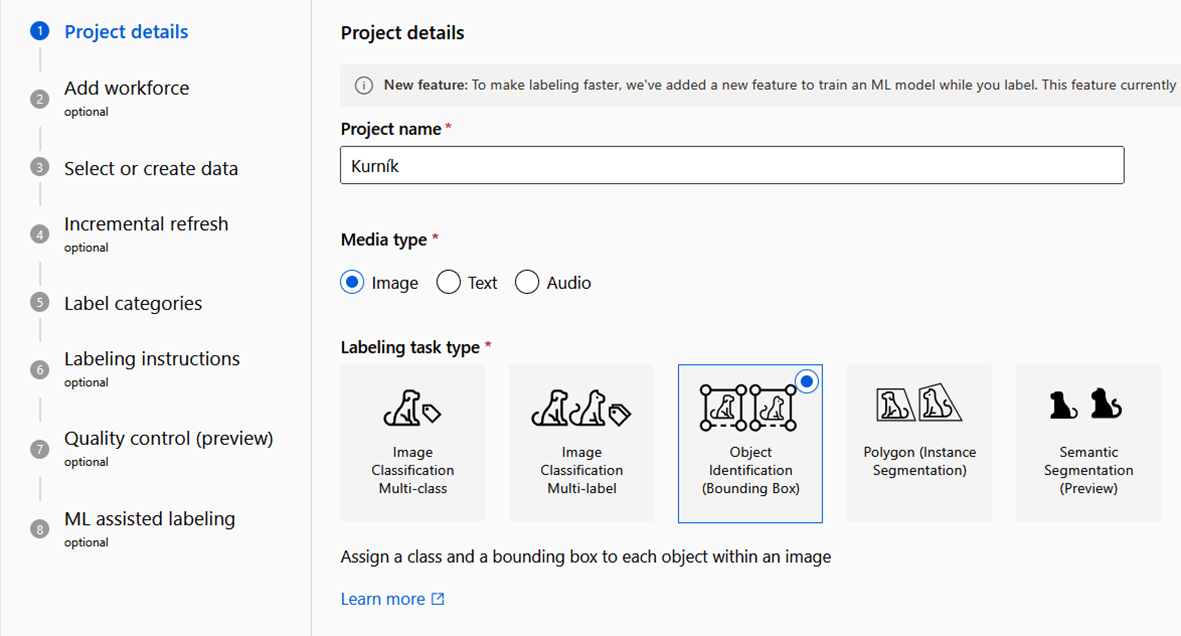
\includegraphics[width=\textwidth]{img/create_learning_project}
    \caption{Vytvoření nového projektu v AML}
    \label{fig:create_learning_project}
\end{figure}


Dále jsem vybral zdroj obrázků, které bylo potřeba klasifikovat.
Vzhledem k tomu, že se jedná o cloudovou službu bylo třeba obrázky slepiček na Azure naimportovat.
Na obrázku~\ref{fig:dataset_selection} je screenshot z Azure Machine Learning studia, kde se zrovna dataset importuje.

\begin{figure}[h]
    \centering
    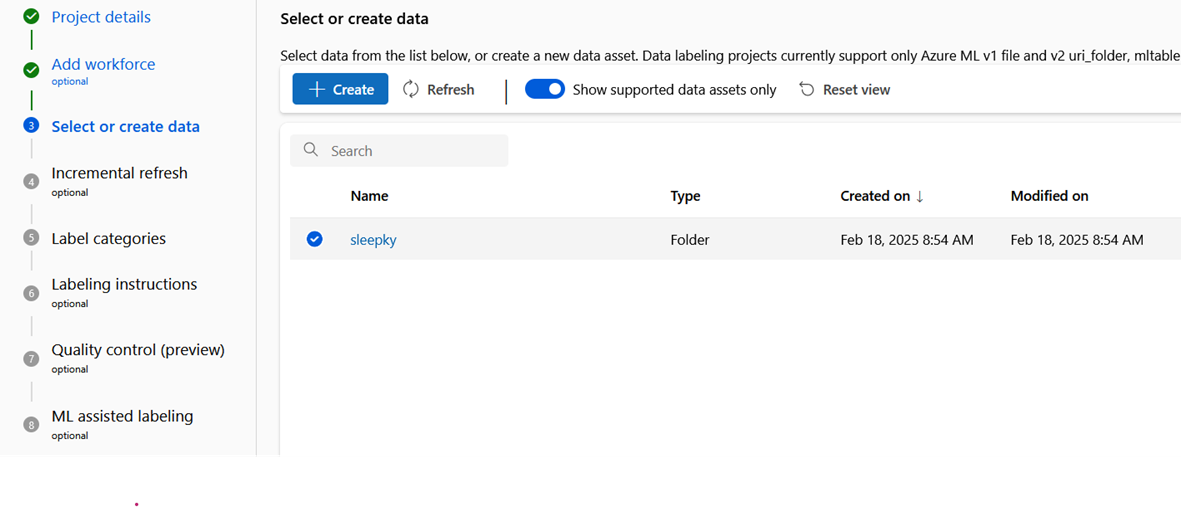
\includegraphics[width=\textwidth]{img/dataset_selection}
    \caption{Tvorba datasetu v AML}
    \label{fig:dataset_selection}
\end{figure}

V dalším kroku jsem nadefinoval kategorie, které budu chtít v obraze identifikovat.
V mém případě jsem zvolil label „slepice“.
Definice kategorií je na obrázku~\ref{fig:category_definition}.

\begin{figure}[h]
    \centering
    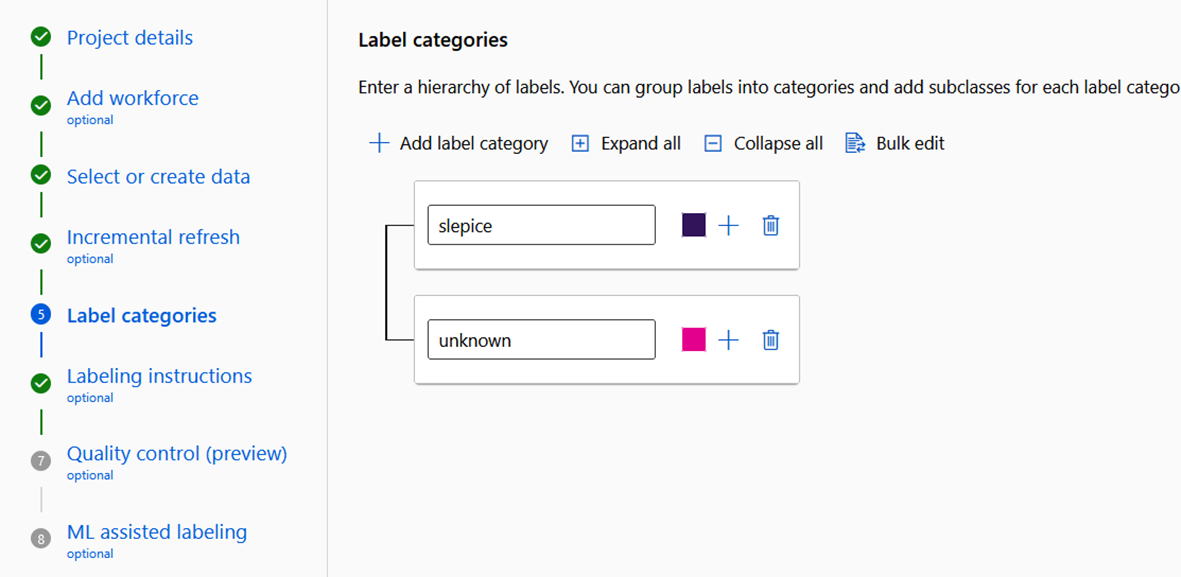
\includegraphics[width=\textwidth]{img/category_definition}
    \caption{Definice kategorií pro učení v AML}
    \label{fig:category_definition}
\end{figure}

V následujícím kroku následovala nejméně zábavná činnost.
Bylo třeba projít jednotlivé snímky a ručně vybrat oblasti, kde já jako člověk vidím slepici.
Oblast, kterou jsem označil se pak následně ukládá jako metadata k obrázku.
Tento proces je znárorněn na obrázku~\ref{fig:chicken_labeling}.

\begin{figure}[h]
    \centering
    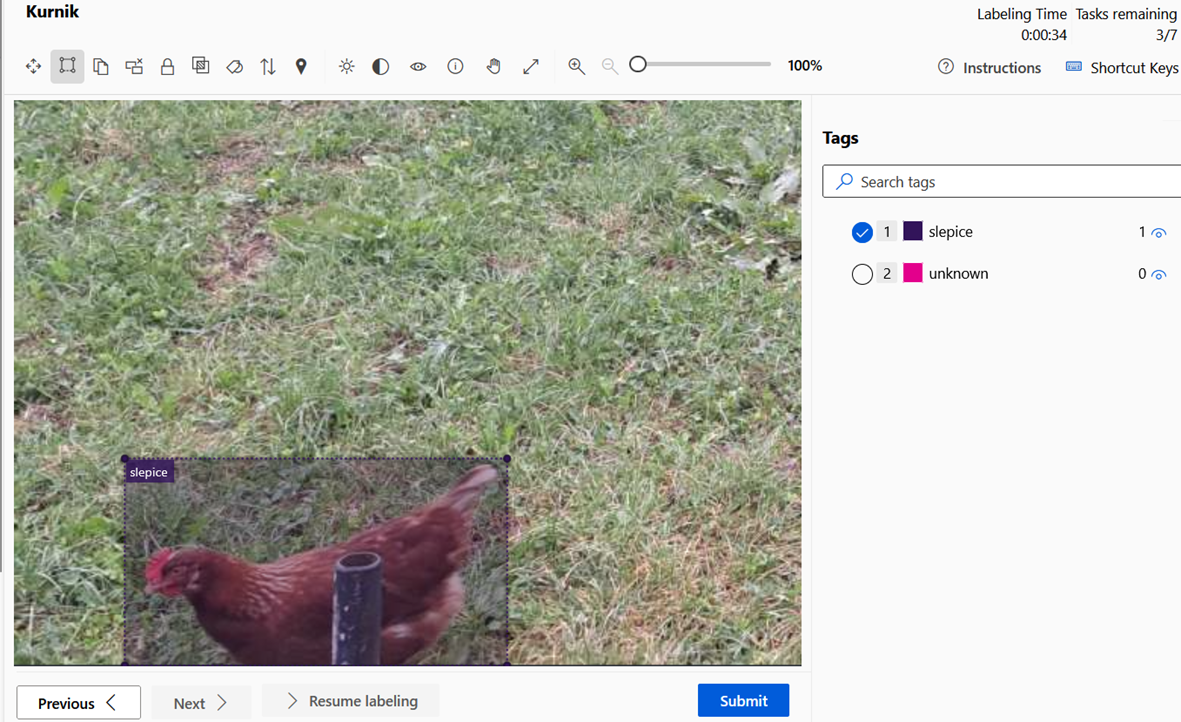
\includegraphics[width=\textwidth]{img/chicken_labeling}
    \caption{Označování slepic pomocí AML}
    \label{fig:chicken_labeling}
\end{figure}

Když se podařilo projít celý obrázkový dataset, mohl jsem vyexportovat „labeling“ data.
Jak jsem psal výše, mít kvalitní učící dataset je důležité, proto jsem exportoval pouze data, která se podařilo úspěšně označit.
Do fotogalerie se mi dostalo i několik nejasných snímků, případně těch, kde slepice nebyla vůbec.
Takové snímky jsem vyřadil.
Anotace jsem exportoval ve formátu COCO => dat odkaz do slovniku
Formát COCO (Common Objects in Context) je standardní formát pro anotaci obrázků používaný ve strojovém učení a počítačovém vidění.
Jeho hlavním cílem je poskytnout strukturu pro uložení informací o objektech v obrázcích, což umožňuje efektivní trénink a hodnocení modelů detekce objektů, segmentace a dalších úloh počítačového vidění.
Obrázek~\ref{fig:create_learning_project} ukazuje jak například může vypadat nastavení pro export COCO formátu z AML.

\begin{figure}[h]
    \centering
    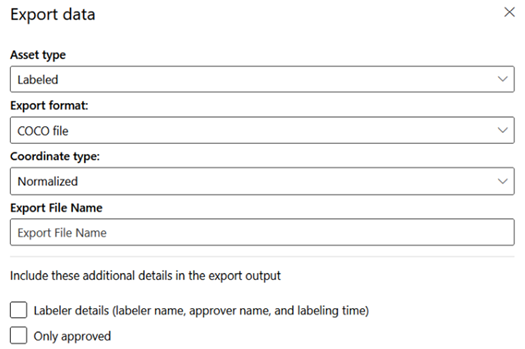
\includegraphics[width=\textwidth]{img/export_coco_format}
    \caption{Export metadat k obrázkům z AML do COCO formátu}
    \label{fig:export_coco_format}
\end{figure}

Soubor obsahuje několik klíčových sekcí: images, annotations, a categories.\newline
Zde je popis jednotlivých částí daného JSON souboru ve formátu COCO:
\begin{enumerate}
    \item images: Tato sekce obsahuje informace o každém obrázku v datasetu.
    \begin{itemize}
        \item id: Unikátní identifikátor obrázku (zde 1).
        \item width a height: Rozměry obrázku (zde 534 pixelů x 291 pixelů).
        \item file\_name: Cesta k souboru obrázku včetně názvu souboru.
        \item coco\_url, absolute\_url: Adresy, kde je obrázek uložen, ať už v cloudovém sandboxu (coco\_url) nebo přes URL pro přímý přístup (absolute\_url).
        \item date\_captured: Čas a datum zachycení obrázku v UTC formátu.
    \end{itemize}
    \item annotations: Tato sekce popisuje anotace neboli poznámky k jednotlivým objektům na obrázcích.
    \begin{itemize}
        \item id: Unikátní identifikátor anotace (zde 1).
        \item category\_id: Odkazuje na kategorii objektu (zde 1, což odpovídá \"slepice\").
        \item image\_id: ID obrázku, na který se tato anotace vztahuje.
        \item area: Relativní plocha objektu na obrázku (zde 0.016).
        Tato hodnota je často normalizována vzhledem k velikosti obrázku.
        \item bbox: Vektor čtyř čísel, který definuje obdélník (bounding box) okolo objektu na obrázku.
        Hodnoty jsou obvykle normalizované, takže se pohybují mezi 0 a 1 a odpovídají relativním souřadnicím a rozměrům (x, y, šířka, výška).
    \end{itemize}
    \item categories: Tato sekce obsahuje seznam kategorií, do kterých mohou objekty na obrázcích patřit.
    \begin{itemize}
        \item id: Unikátní identifikátor kategorie.
        \item name: Jméno nebo popis kategorie (zde \"slepice\" a \"unknown\").
    \end{itemize}
\end{enumerate}

Tento JSON tedy popisuje dataset obsahující obrázek s jedním označeným objektem, který patří do kategorie \"slepice\".
COCO formát umožňuje uložení komplexních a strukturovaných dat o objektech na obrázcích, což je velmi užitečné pro trénování a testování modelů strojového učení.
Příklad tohoto formátu metadat pro strojové učení je na obrázku~\ref{fig:coco_format}.

\begin{figure}[h]
    \centering
    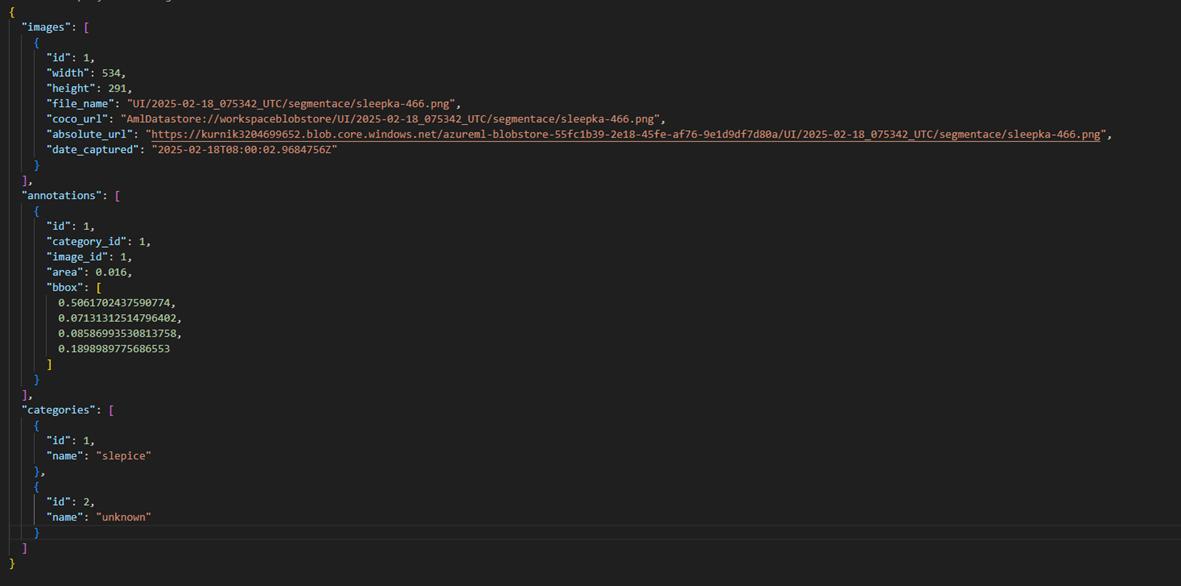
\includegraphics[width=\textwidth]{img/coco_format}
    \caption{Vytvoření nového projektu v AML}
    \label{fig:coco_format}
\end{figure}

\subsubsection{Doučování modelu Yolov11 o novou třídu}
V předchozí sekci jsem si popsali jak vytvořit zdroje dat a nyní jsme připraveni, vyučit existující model.
Doučovat doma existující model je relativně složité, ale díky výborné dokumentaci na strankach https://docs.ultralytics.com/ jsem to zvladnul.
Základem pro úspěšné a efektivní učení je hardware.
Hlavně GPU, protože trénování modelů hlubokého učení je výpočetně náročné.
Vypozoroval jsem, že největší vliv na učení má velikost paměti grafické karty.
V mém případě byla použita Nvidia RTX 4070.
O stavbě a následném učení neuronových sítí by se nechalo desítky stránek, ale to není předmětem mojí práce.
Rád bych alespon představil blokové schema učícího procesu.\newline
\newline
Pro učení jsem použil script, ktery jsem si pripravil.
Volání jednotlivých kroků pro učení je znázorněno na screenshotu učící metody na obrázku~\ref{fig:learn_script}

\begin{figure}[h]
    \centering
    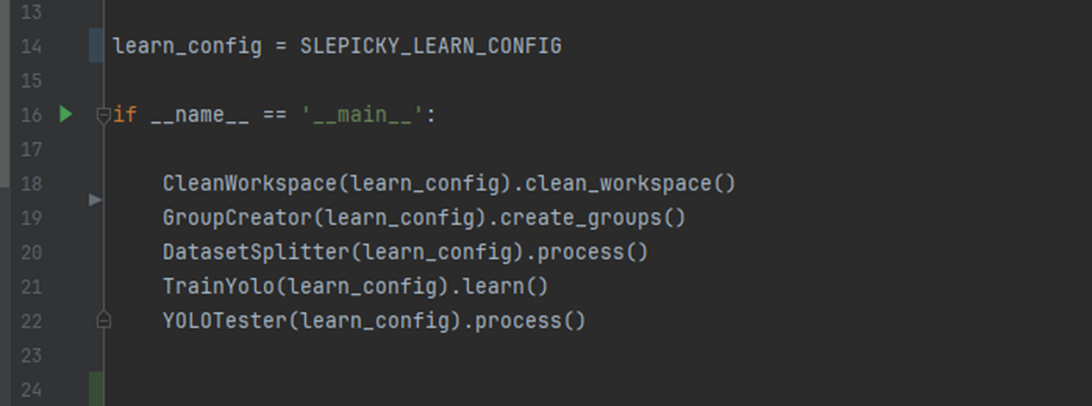
\includegraphics[width=\textwidth]{img/learn_script}
    \caption{Vytvoření nového projektu v AML}
    \label{fig:learn_script}
\end{figure}

\paragraph{Krok 1 - CleanWorkspace}

Tento krok je zodpovědný za přípravu pracovního prostředí před zahájením tréninkového procesu.
Odstranuji v něm archivaci stávajících dat a modelů, které mi ve workspace zůstaly z předchozich běhů a již nejsou potřebné.
Čištění pomáhá zabránit kolizím s předchozími seancemi a udržet v něm pořádek, což zajišťuje, že nové modely a datové soubory jsou aktuální a správně organizované.

\paragraph{Krok 2 - GroupCreator}

Tento krok se zaměřuje na organizaci dat do různých skupin pro trénování a testování modelu.
Data mám rozdělena v několika různých adresářích a tento krok má na starost jejich správné složení.
Stejná data používám výuků modelu na počítání slepic, detekce vetřelce a plánované reidentifikace slepic.

\paragraph{Krok 3 - DatasetSplitter}

Proces rozdělení datasetu je klíčový pro oddělení trénovací, validační a testovací sady.
Rozdělení může být prováděno v daných poměrech, například 70% trénovací data, 15% validační data a 15% testovací data.
Správné rozdělení dat je důležité pro zajištění objektivního hodnocení modelu, aby se předešlo přeškolení.
Tento krok také zajišťuje, že žádné datové soubory nejsou opominuty a že rozdělení je náhodné a reprezentativní.

\paragraph{Krok 4 - TrainYolo}

Jedná se o hlavní krok, kde je model YOLOv11 trénován na trénovacích datech.
Proces zahrnuje několik iterací (epoch) přes trénovací data, během kterých model aktualizuje své váhy podle chybného odhadu.
Na obrázku~\ref{fig:train_yolo}.


\begin{figure}[h]
    \centering
    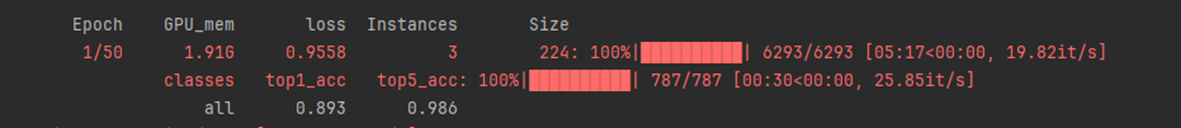
\includegraphics[width=\textwidth]{img/train_yolo}
    \caption{Proces trénování YOLOv11 modelu}
    \label{fig:train_yolo}
\end{figure}

Během trénování se sleduje výkonnost modelu na validačních datech, která zabraňují přeškolení.
Přeškolení si můžeme představit například u modelu, který rozpoznává kačeny, kočky a slepice.
I když všechny konfigurační parametry byly správně,  systém v některých případech špatně identifikoval kočku.
Až zpětnou analýzou trénovacích dat bylo zjištěno, že došlo k přeškolení.
System identifikoval kachnu nikoliv podle tvaru jejího těla, případně zabarvení, jako to udělá člověk, ale podle toho, zda na obrázku byla ci nebyla tráva.
To pak vedlo k tomu, že pokud byla kočka na trávě, byla označena za kachnu.
Spusti trénovací smyčku je jednoduché.
Bylo třeba předat jen několik základních parametrů.
\newline
Training Parameters\newline
Epochs: 50\newline
Batch Size: 16\newline
Pretrained: True (using pretrained weights)\newline
Data Path: c:/kurnik/klasifikace/kurnik\_learn\_temp/train\newline

50 Epoch známená kolik poběží učících cyklů.\newline
Batch Size – specifikuje kolik vláken poběží paralelně, je třeba dbát na velikost pameti grafické karty\newline
Pretrained – říká, že budeme rozšiřovat již naučený model\newline
Data Path – specifikuje odkud se mají vzit data k učeni.\newline

\paragraph{Krok 5 - YOLOTester:}

Po úspěšném tréninku modelu je nutné jeho testování na dříve oddělené testovací sadě.
Tento krok zahrnuje vyhodnocení výkonnosti modelu pomocí metrik, jako je přesnost, citlivost.
Testování nám poskytuje objektivní zpětnou vazbu o tom, co za objekty model umí ve snímcích rozpoznat. Důležíté je předkladat pro testování snímky, které během tréninku neviděl.
Na základě testovacích výsledků jsem pak následně prováděl úpravy učicích parametrů, případně jsem dodával další data do učícího datasetu.

\begin{figure}[h]
    \centering
    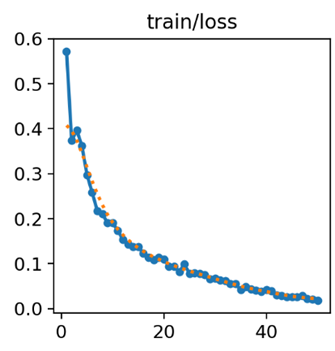
\includegraphics[width=\textwidth]{img/loss_funkce}
    \caption{Graf loss funkce v závyslosti na počtu etap}
    \label{fig:loss_funkce}
\end{figure}

Graf který je automaticky generováný při učení nám umožnuje sledovat, jak dobře se model učí vzhledem k časové ose tréninku.
Tento graf typicky zobrazuje ztrátovou funkci (loss) na svislé ose (Y) a počet trénovacích epoch nebo kroků na vodorovné ose (X).

\begin{figure}[h]
    \centering
    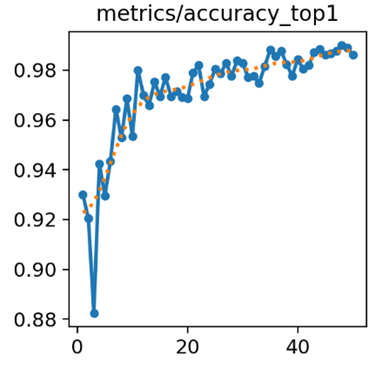
\includegraphics[width=\textwidth]{img/top1_accuracy}
    \caption{Vytvoření nového projektu v AML}
    \label{fig:top1_accuracy}
\end{figure}

Tento graf se zaměřuje na metriku přesnosti, konkrétně na \"top-1 accuracy,\" která měří, jak často je nejpravděpodobnější (nejvyšší hodnocená) předpověď modelu správná.

Výsledky detekce jsou demostrovány na obrázcích~\ref{fig:chicken_detection1},~\ref{fig:chicken_detection2},~\ref{fig:chicken_detection3},~\ref{fig:chicken_detection4},

\newpage
\begin{figure}[h]
    \centering
    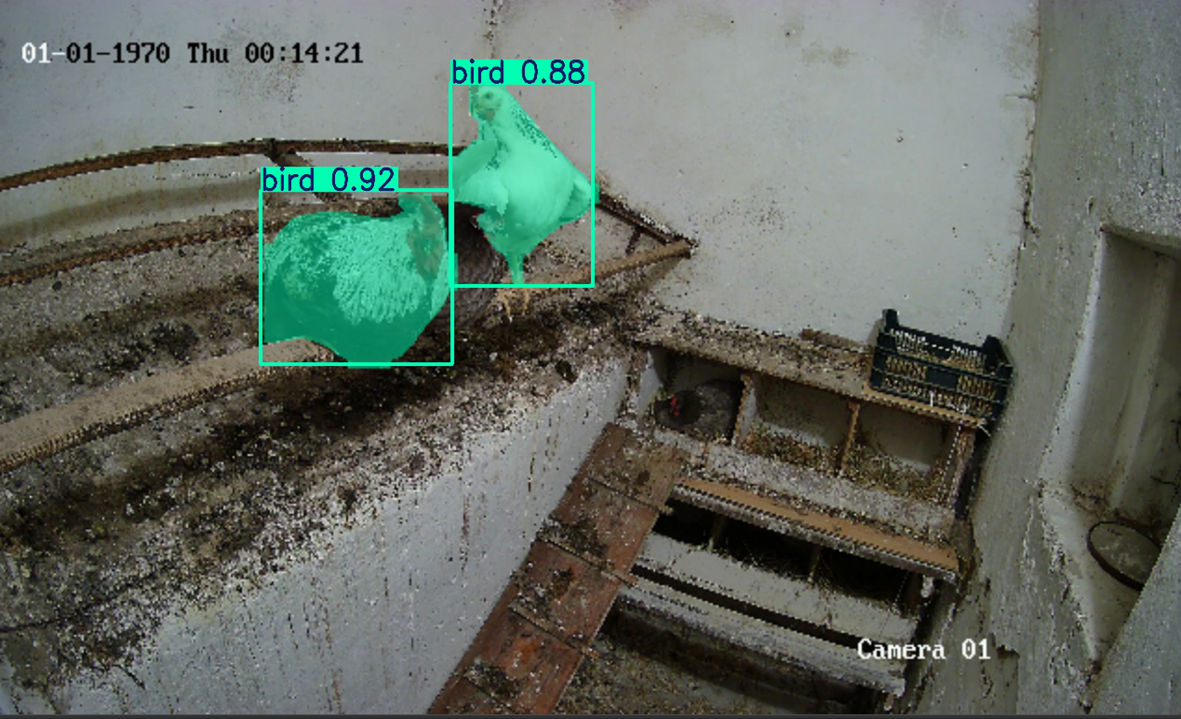
\includegraphics[width=\textwidth]{img/chicken_detection1}
    \caption{Ukázka výsledné detekce slepic v obraze 1}
    \label{fig:chicken_detection1}
\end{figure}
\begin{figure}[h]
    \centering
    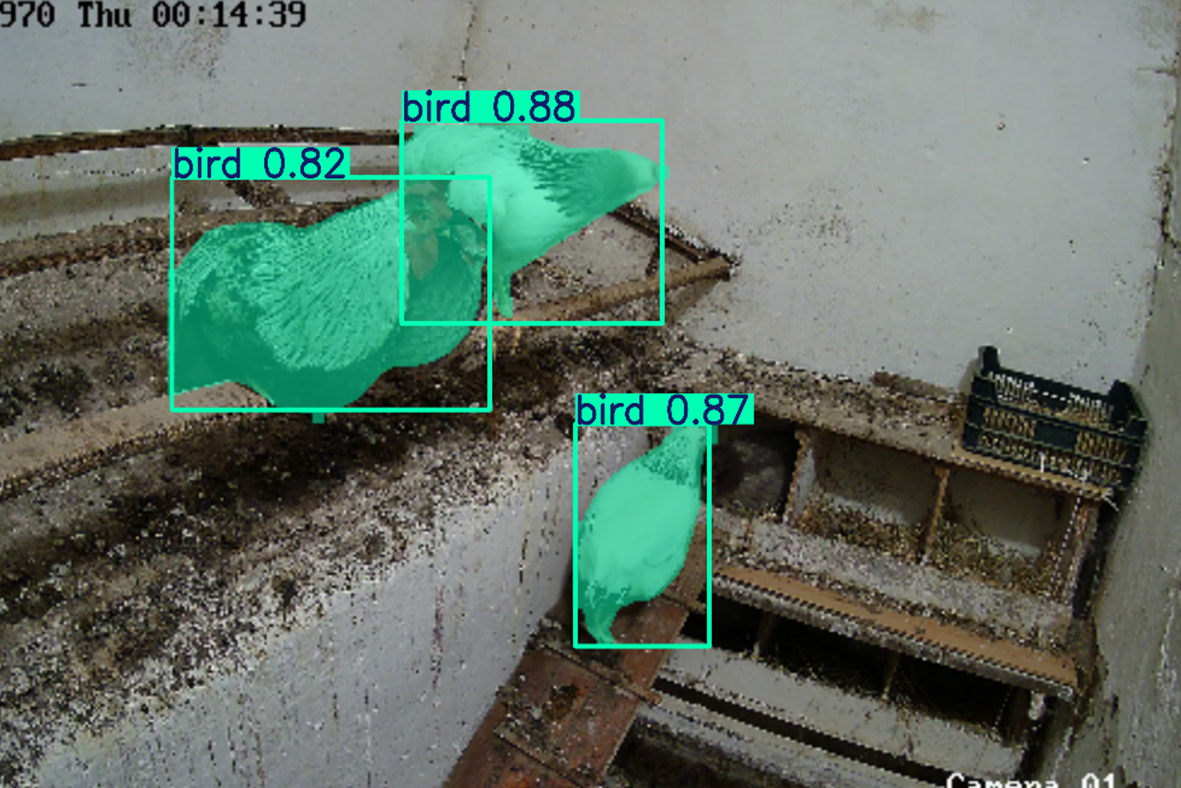
\includegraphics[width=\textwidth]{img/chicken_detection2}
    \caption{Ukázka výsledné detekce slepic v obraze 2}
    \label{fig:chicken_detection2}
\end{figure}
\newpage
\begin{figure}[h]
    \centering
    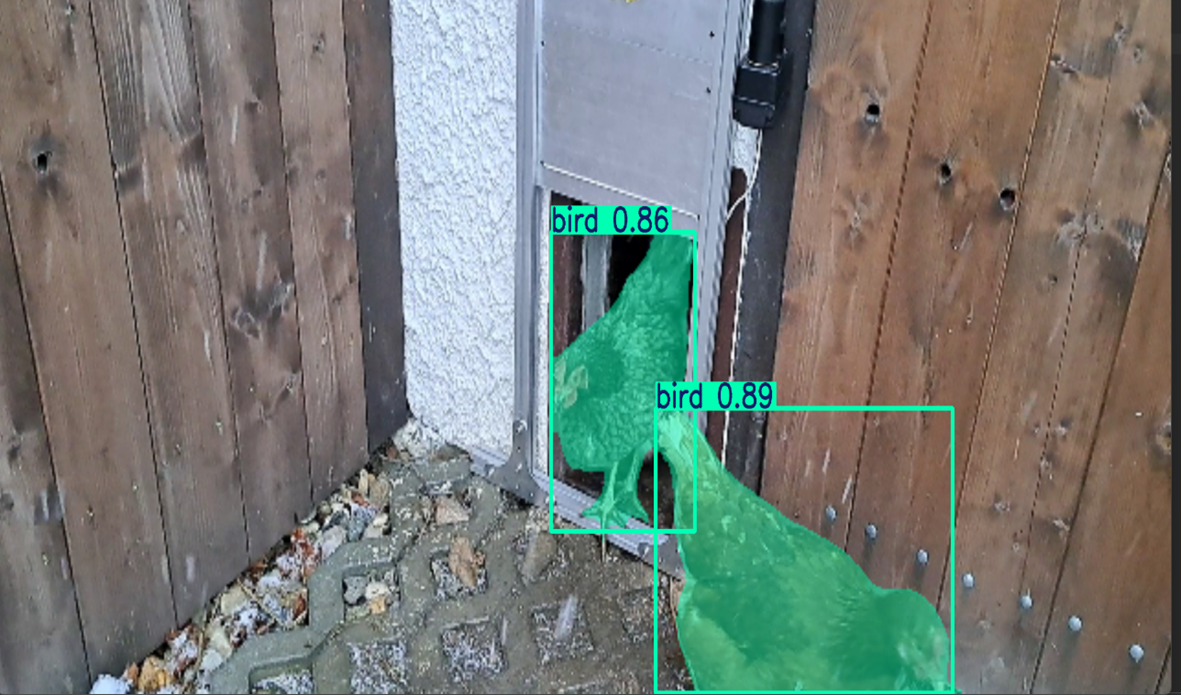
\includegraphics[width=\textwidth]{img/chicken_detection3}
    \caption{Ukázka výsledné detekce slepic v obraze 3}
    \label{fig:chicken_detection3}
\end{figure}
\begin{figure}[h]
    \centering
    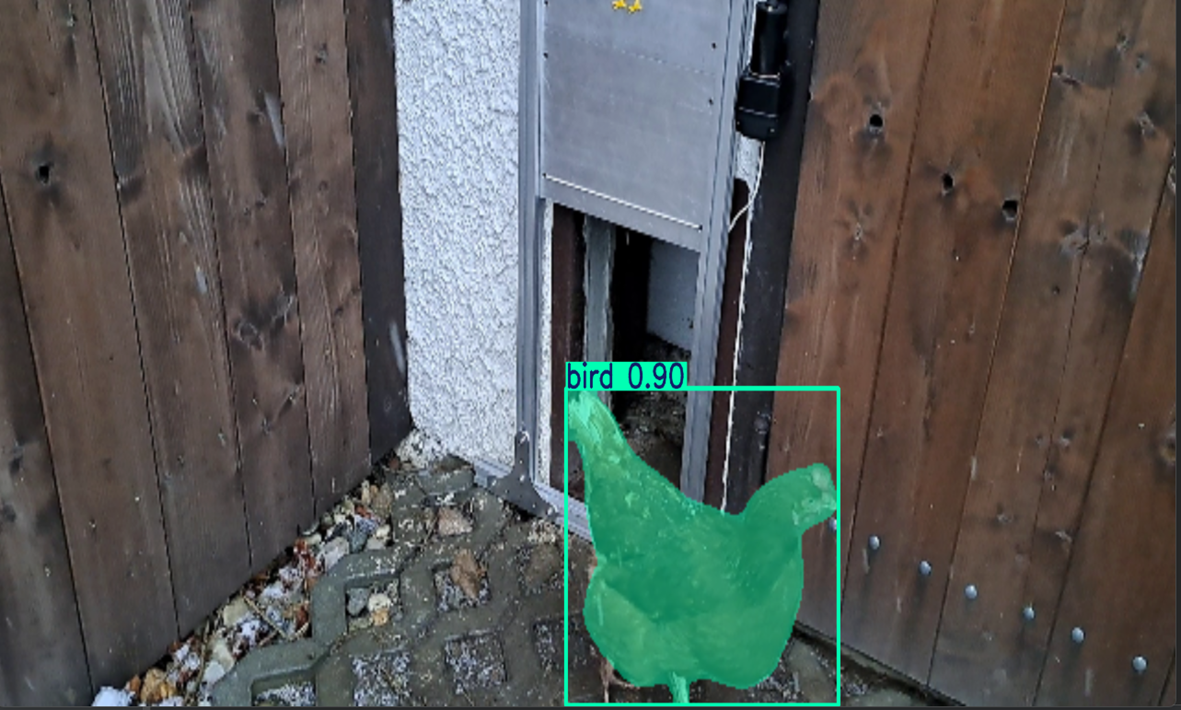
\includegraphics[width=\textwidth]{img/chicken_detection4}
    \caption{Ukázka výsledné detekce slepic v obraze 4}
    \label{fig:chicken_detection4}
\end{figure}
\newpage

%todo fix render obrázků